\chapter{Integration strategy}


\section{Entry criteria}
Before the integration testing phase proper may begin, it is important that the code has been inspected, manually or otherwise, and that unit tests have been run, so that any bug or issue found in this phase may be safely flagged as being a problem of integration and not something that works as it shouldn't at a lower level.


\section{Elements to be integrated}
\begin{figure}
\centering
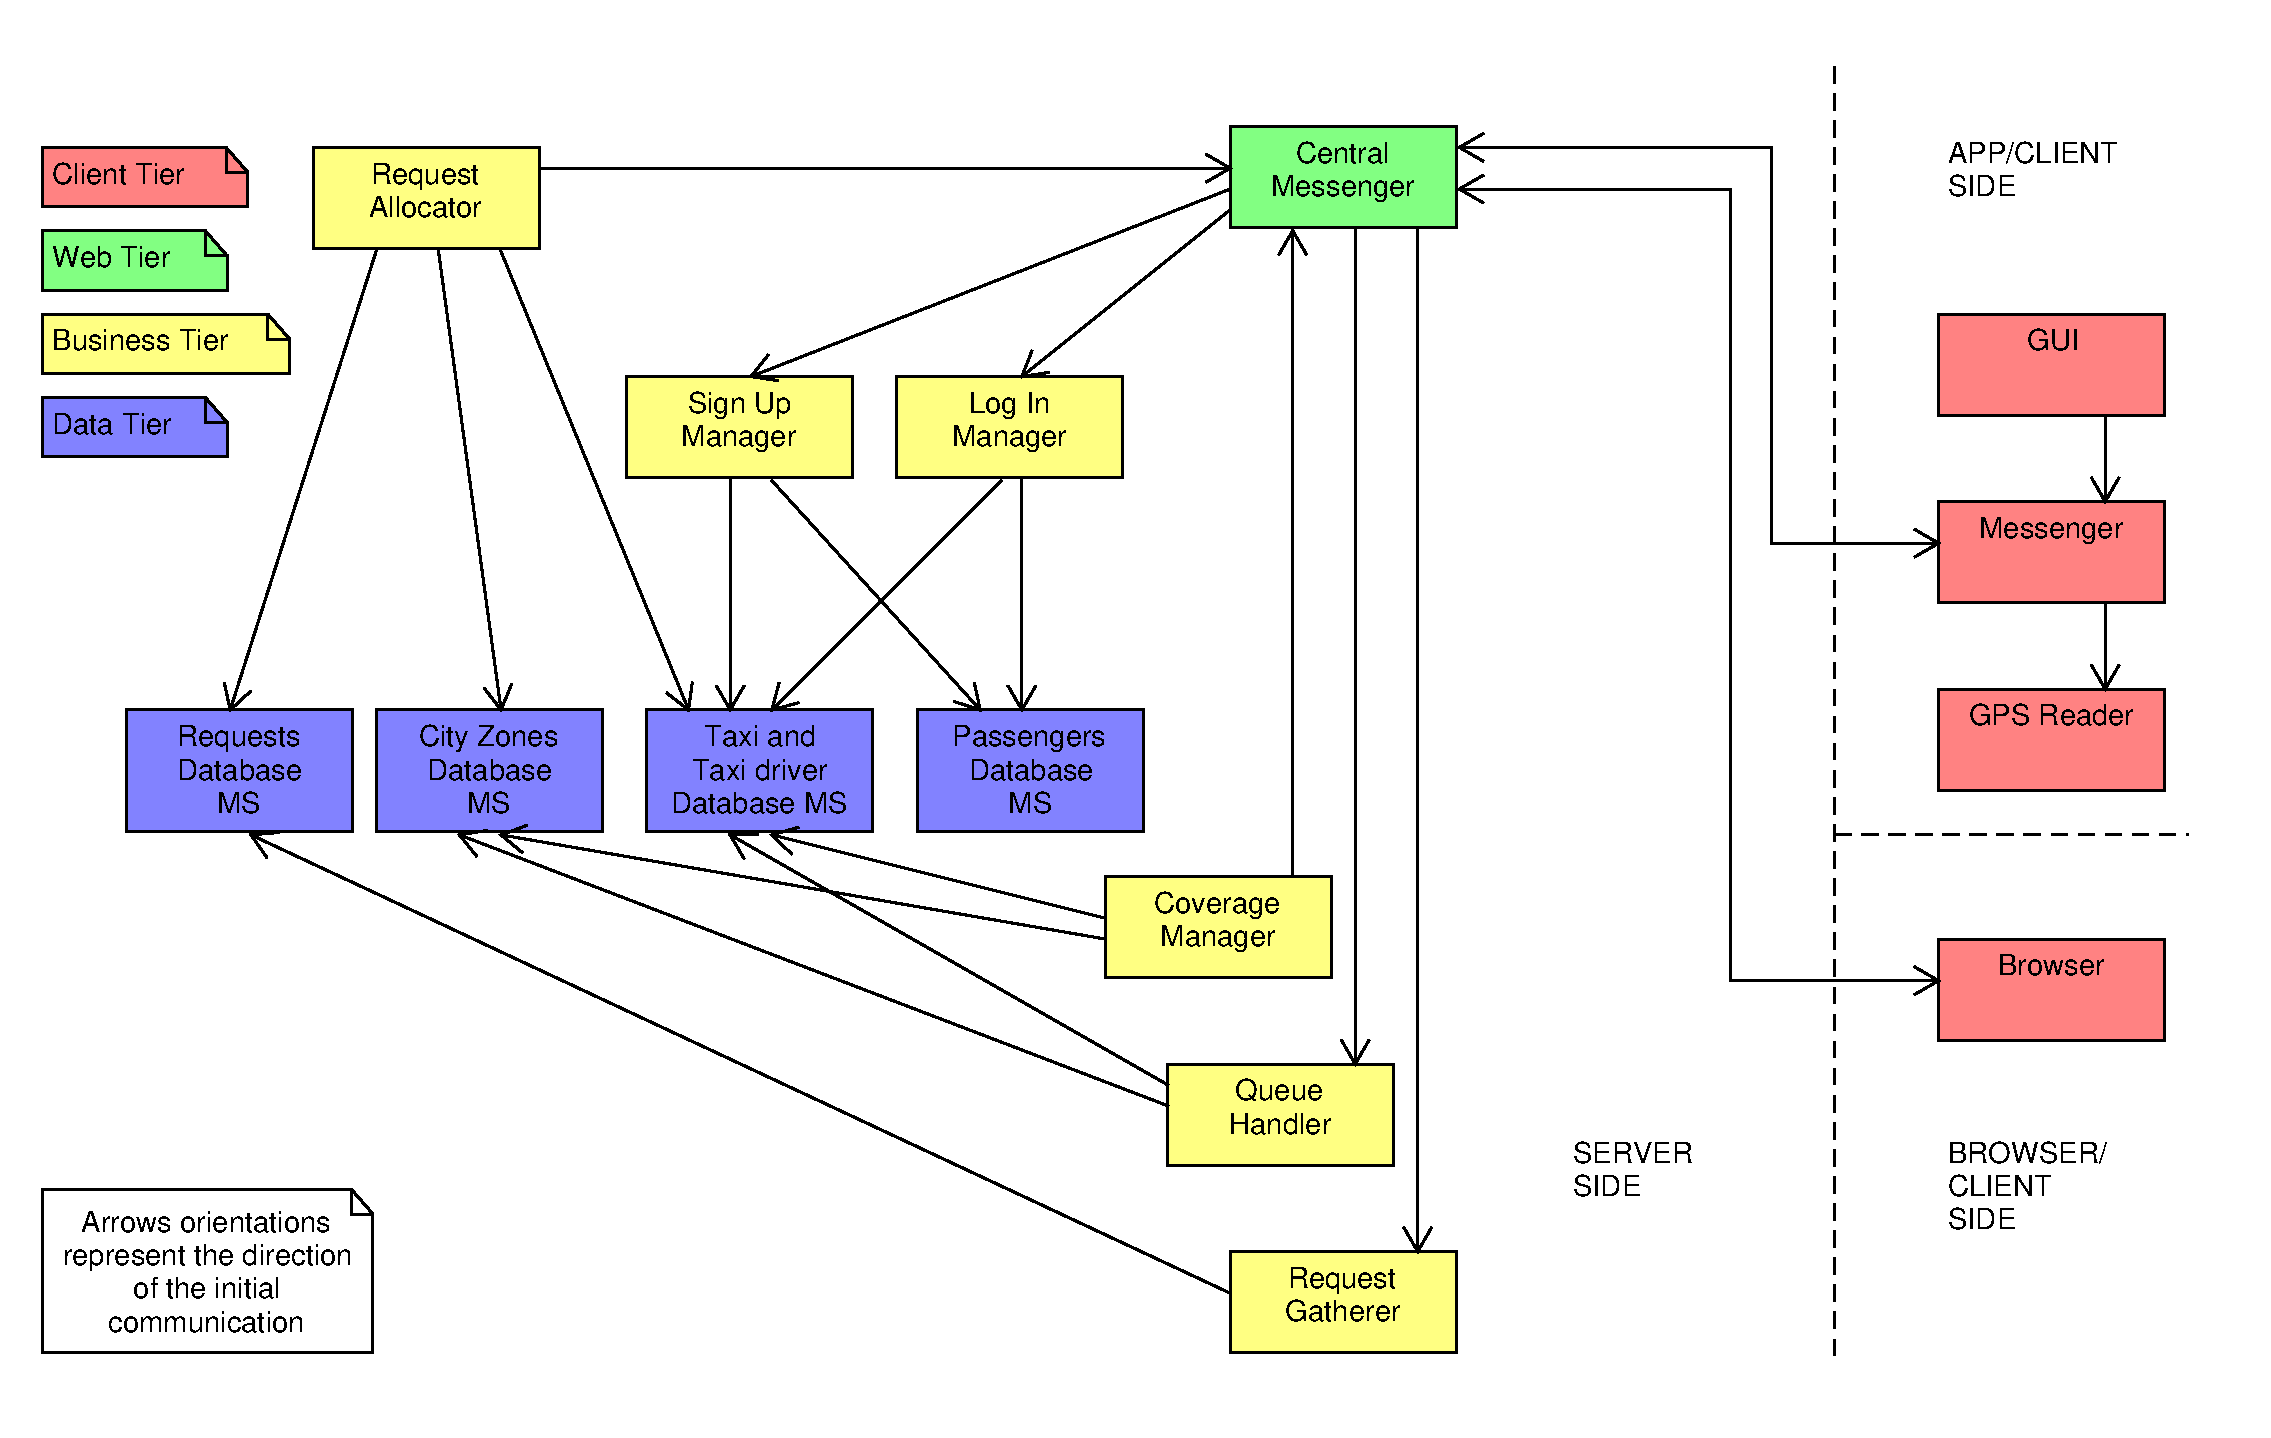
\includegraphics[width=\textwidth]{tex-images/interactions}
\caption{The different architectural components and their interaction -- see the \emph{Design Document}}
\end{figure}
As detailed in the \emph{Design Document}, the architecture is organized in several higher level components themselves divided in lower level modules. Refer to the \emph{Design Document} itself for a detailed description of the elements.

\subsection{Client Tier}
\subsubsection{Central Messenger}
\begin{itemize}
\item [A1] A module that interfaces with GUI;
\item [A2] A module that interfaces with GPS Reader;
\item [A3] A module that interfaces with Server Central Messenger;
\item [A4] A module that handles and forwards messages to modules.
\end{itemize}

\subsubsection{GPS Reader}
\begin{itemize}
\item [B1] A module that interfaces with Central Messenger in order to receive requests and send information;
\item [B2] A module that reads GPS information from Mobile APIs.
\end{itemize}

\subsubsection{Graphical User Interface}
\begin{itemize}
\item [C1] A module that interfaces with Central Messenger in order to receive and send messages;
\item [C2] A module that shows navigation pages.
\end{itemize}

\subsection{Web Tier}
\subsubsection{Central Messenger}
\begin{itemize}
\item [D1] A module that interfaces with Queue handler;
\item [D2] A module that interfaces with Request Allocator;
\item [D3] A module that interfaces with Request Gatherer;
\item [D4] A module that interfaces with Coverage Manager;
\item [D5] A module that interfaces with Sign Up/Log In manager;
\item [D6] A module that interfaces with Client Central Messenger;
\item [D7] A module that interfaces with Client Browser;
\item [D8] A module that handles and forward messages throw modules.
\end{itemize}


\subsection{Business Tier}
\subsubsection{Sign Up Manager}
\begin{itemize}
\item [E1] A \emph{Communication module} that interfaces with Central Messenger;
\item [E2] An \emph{Analysis module} that, reading form \emph{Data module}, analyses the correctness of data and it eventually confirms or rejects;
\item [E3] A \emph{Data module} that stores data in the correct database and read needed information.
\end{itemize}

\subsubsection{Log In Manager}
These modules perform exactly as the Sign Up Manager, so their functional integration testing is handled in the exact same way.
\begin{itemize}
\item [E1] A \emph{Communication module} that interfaces with Central Messenger:
\item [E2] An \emph{Analysis module} that, reading form \emph{Data module}, analyses the correctness of data and it eventually confirms or rejects;
\item [E3] A \emph{Data module} that stores data in the correct database and read needed information.
\end{itemize}

\subsubsection{Coverage Manager}
\begin{itemize}
\item [F1] A \emph{Data module} that interfaces with databases making DBMS queries;
\item [F2] An \emph{Analysis module} that analyses information received from \emph{Data module} and calculates the best coverage;
\item [F3] A \emph{Communication module} that interfaces with Central Messenger in order to send messages to Taxi Drivers selected by \emph{Analysis module}.
\end{itemize}

\subsubsection{Request Gatherer}
\begin{itemize}
\item [G1] A \emph{Communication module} that receives requests messages from Central Messenger;
\item [G2] An \emph{Analysis Module} that analyses data integrity and requests information received from \emph{Communication module} and eventually it sends to \emph{Data Module};
\item [G3] A \emph{Data Module} that stores information interfacing with databases.
\end{itemize}

\subsubsection{Request Allocator}
\begin{itemize}
\item [H1] A \emph{Data Module} that, periodically reading from databases, controls if there are requests to fulfil and updates taxi drivers’ information;
\item [H2] An \emph{Analysis module} that choses taxi diver to allocate to the requests;
\item [H3] A \emph{Communication module} that interfaces with Central Messenger in order to send notifications to taxi drivers.
\end{itemize}

\subsubsection{Queue Handler} 
\begin{itemize}
\item [I1] A \emph{Communication module} that receives availability messages from Central Messenger;
\item [I2] A \emph{Data module} that store and updates information in database.
\end{itemize}


\section{Integration testing strategy}
Since, as stated, the high level components are divided in low level modules, it is at first necessary to test the integration of the modules that make a single component before that same component can be tested against the others at the higher level.

A top down approach will be followed for the integration of the components. The process is very much simplified by the almost complete independence of most of the different components. As for the modules, since their number is rather small, a top down or functional grouping approach can be used indifferently without much impact overall.


\section{Sequence of integration}

\subsection{Components}
Since a top down (from the interface) approach will be used, the integration order will be as follow:
\begin{enumerate}
\item Client App GUI;
\item Client App Messenger;
\item Client App GPS Reader;
\item Client Webapp (on par with the three previous components);
\item Central messenger;
\item Log in manager;
\item Sign up magager;
\item Request allocator;
\item Coverage manager;
\item Queue handler;
\item Request gatherer;
\item All Database Management Systems.
\end{enumerate}

\subsection{Modules}
